\documentclass[10pt]{article}
\usepackage[margin=0.62in]{geometry}
\usepackage[T1]{fontenc}
\usepackage{lmodern,microtype}
\usepackage{booktabs,tabularx,array,graphicx}
\usepackage{xcolor,amsmath,amssymb}
\usepackage{tikz}
\usetikzlibrary{arrows.meta,positioning,fit}
\usepackage{pgfplots}
\usepgfplotslibrary{groupplots}
\pgfplotsset{compat=1.18}
\usepackage[most]{tcolorbox}
\usepackage{enumitem}
\usepackage[hidelinks]{hyperref}

\definecolor{navy}{HTML}{17365D}
\definecolor{blue}{HTML}{2F75B5}
\definecolor{teal}{HTML}{1B998B}
\definecolor{orange}{HTML}{E67E22}
\definecolor{red}{HTML}{B03A2E}
\definecolor{green}{HTML}{2E7D32}
\definecolor{pale}{HTML}{F3F6FA}
\definecolor{rulegray}{HTML}{D5DBE3}
\setlength{\parindent}{0pt}
\setlength{\parskip}{3pt}
\setlist[itemize]{leftmargin=5mm,itemsep=2pt,topsep=2pt}
\renewcommand{\arraystretch}{1.10}
\newcommand{\NA}{\textemdash}
\newtcolorbox{infobox}[1][]{enhanced,boxrule=0.6pt,colback=pale,colframe=rulegray,
  arc=1.5mm,left=2mm,right=2mm,top=1.2mm,bottom=1.2mm,#1}

\begin{document}
\begin{center}
{\LARGE\bfseries\color{navy} 602 Direct-Action LSTM vs. Offline SPP}\\[2pt]
{\small 602.gcc\_s-734B \quad $\vert$ \quad seed 7 \quad $\vert$ \quad 25M measured instructions}\\[4pt]
\fcolorbox{green}{green!7}{\strut\bfseries PASS: fair-input and replay contracts}
\quad
\fcolorbox{red}{red!6}{\strut\bfseries No composite score; dimensions remain separate}
\end{center}

\begin{infobox}
\begin{tabularx}{\textwidth}{@{}>{\bfseries}lX@{}}
Primary comparison & Offline SPP actions versus independently generated LSTM actions, replayed through the same PC--line--occurrence transport and measured against the same no-prefetch baseline.\\
Shared external input & Chronological \texttt{DEMAND(address)} and \texttt{CACHE\_FILL(evicted-address)} callbacks---the source-effective external callback stream audited from SPP.\\
Neural history & One stateful LSTM over complete train--guard--evaluation chronology; chronological TBPTT carries and detaches hidden/cell state.\\
Excluded at inference & PC, cycle, hit/miss, queue state, SPP candidates/actions, confidence, private tables/GHR/filter state, request budget/degree, teacher actions, future rows, and probability thresholds.\\
Action space & Learned zero/positive categorical mode, learned unbounded positive count, autoregressive signed cache-line delta mixture, and learned \texttt{FILL\_L2}/\texttt{FILL\_LLC}; no fixed page-offset interface or neural degree cap.\\
Run artifact & \texttt{602\_offline\_lstm\_spp\_empirical\_prior\_hurdle\_free\_running\_v2\_seed7}. PASS certifies the experiment contract; it does not certify every capacity point.\\
Analyzer outputs & \texttt{matched\_comparison.csv/json} contain raw ChampSim lifecycle counters, event-audit counters, behavior diagnostics, and every separate metric used below. The legacy composite field is deliberately not used.\\
\end{tabularx}
\end{infobox}

\section*{1. What is measured}
\begin{center}
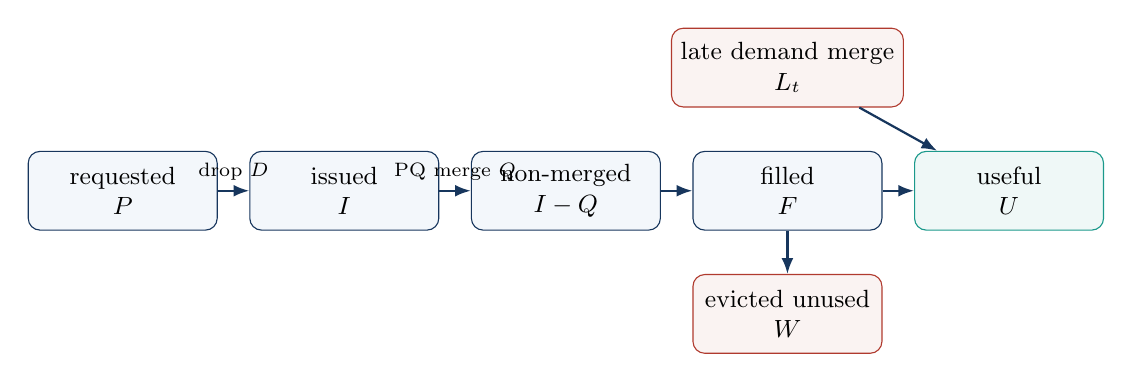
\begin{tikzpicture}[
  node distance=5.5mm and 4mm,
  every node/.style={font=\small},
  counter/.style={draw=navy,rounded corners=1.5mm,fill=blue!6,minimum width=24mm,minimum height=10mm,align=center},
  outcome/.style={draw=teal,rounded corners=1.5mm,fill=teal!7,minimum width=24mm,minimum height=10mm,align=center},
  bad/.style={draw=red,rounded corners=1.5mm,fill=red!6,minimum width=24mm,minimum height=10mm,align=center},
  arrow/.style={-{Latex[length=2mm]},thick,draw=navy}
]
\node[counter] (req) {requested\\$P$};
\node[counter,right=of req] (iss) {issued\\$I$};
\node[counter,right=of iss] (uniq) {non-merged\\$I-Q$};
\node[counter,right=of uniq] (fill) {filled\\$F$};
\node[outcome,right=of fill] (use) {useful\\$U$};
\node[bad,below=of fill] (waste) {evicted unused\\$W$};
\node[bad,above=of fill] (late) {late demand merge\\$L_t$};
\draw[arrow] (req)--node[above,font=\scriptsize]{drop $D$} (iss);
\draw[arrow] (iss)--node[above,font=\scriptsize]{PQ merge $Q$} (uniq);
\draw[arrow] (uniq)--(fill);
\draw[arrow] (fill)--(use);
\draw[arrow] (fill)--(waste);
\draw[arrow] (late)--(use);
\end{tikzpicture}
\end{center}

\begin{minipage}[t]{0.49\textwidth}
\begin{infobox}[title={\bfseries Outcome and reach}]
\[
m=\frac{M}{N_L},\quad
S=\frac{\mathrm{IPC}}{\mathrm{IPC}_0},\quad
R_m=\frac{M_0-M}{M_0},\quad
C=\frac{U}{M_0}.
\]
$N_L$ and $M$ are measured L2 loads and misses; subscript 0 denotes no prefetch. $C$ is useful-prefetch coverage against no-prefetch misses, while $R_m$ is observed miss reduction. They are related but not interchangeable.
\end{infobox}
\end{minipage}\hfill
\begin{minipage}[t]{0.49\textwidth}
\begin{infobox}[title={\bfseries Accuracy, timeliness, and pressure}]
\[
A=\frac{U}{I},\quad
A_{\rm sel}=\frac{U}{I-Q},\quad
T=\frac{U}{U+L_t},\quad
\rho=\frac{P}{N_L}.
\]
$A_{\rm sel}$ removes PQ-merged duplicates from the denominator. It is not a pollution metric. $T$ asks whether useful requests arrived before demand; $\rho$ exposes request pressure.
\end{infobox}
\end{minipage}

\begin{infobox}[title={\bfseries Exact interpretation boundaries}]
The analyzer obtains $N_L,M,P,D,I,Q,F,U,W,$ and $L_t$ from the recorded
ChampSim measurement counters and retains the event stream as an independent
cross-check. No value below is inferred from a CSV field name. Source audit
confirms that $U$ increments on the first read hit to a prefetched line and
clears its prefetch bit; $W$ increments when a still-prefetched, unused line is
replaced; $F$ increments when a prefetch is filled; $L_t$ increments when
demand merges into an in-flight prefetch; and $Q$ increments for a duplicate
in the prefetch queue. A zero denominator is reported as \NA, not as evidence
of 0\% accuracy or timeliness. We additionally report $U/M$, $Q/I$, $D/P$,
$F/(I-Q)$, $L_t/I$, $W/I$, and resolved-fill utility $U/(U+W)$.
Hennessy and Patterson motivate keeping these dimensions separate: bad
prefetches may displace useful blocks and consume bandwidth, while useful
prefetches must arrive in time and avoid excessive outstanding
work.\footnote{J. L. Hennessy and D. A. Patterson, \emph{Computer
Architecture: A Quantitative Approach}, 7th ed., Sec.~2.3, pp.~127--129;
Exercise~2.3, p.~160.} No harmful-victim plus later-re-reference counter is
recorded. Therefore $W$ and request pressure indicate risk, but neither is
renamed cache pollution and no aggregate score is reported.
\end{infobox}

\subsection*{Held-out callback decision audit}
\begin{infobox}[title={\bfseries Dense teacher, always-act student}]
SPP's chronological evaluation stream contains demand and cache-fill
callbacks, but the decision denominator here is exactly the $404{,}219$
held-out \emph{demand} callbacks.  A callback is \emph{act} when $K>0$, not
when it emits exactly one action.  The SPP teacher is 97.24\% act/2.76\%
silent; every tested LSTM capacity is 100\% act/0\% silent.  Trigger-confusion
counters show 2.76\% silent$\to$act and 0.00\% act$\to$silent.  These are
imitation outcomes, not useful/harmful classifications; cache outcomes are
measured separately by replay.
\end{infobox}

\begin{center}\scriptsize
\begin{tabular}{@{}lrrrrrrr@{}}
\toprule
Capacity & SPP silent & SPP act & LSTM silent & LSTM act &
$\Delta$ act (pp) & silent$\to$act & act$\to$silent \\
\midrule
h8--h128 & 2.76\% & 97.24\% & 0.00\% & 100.00\% &
+2.76 & 2.76\% & 0.00\% \\
\bottomrule
\end{tabular}
\end{center}

\section*{2. Cache outcomes}
\begin{center}\scriptsize
\resizebox{\textwidth}{!}{%
\begin{tabular}{@{}lrrrrrrrr@{}}
\toprule
Method & params & cycles & IPC & speedup & L2 loads & L2 misses & miss rate & miss reduction \\
\midrule
No prefetch & -- & 67.935M & 0.36800 & 1.0000 & 404,219 & 203,131 & 50.25\% & 0.00\% \\
Offline SPP & -- & 58.365M & 0.42834 & 1.1640 & 404,219 & 70,874 & 17.53\% & 65.11\% \\
Live SPP (context) & -- & 58.362M & 0.42836 & 1.1640 & 404,219 & 70,873 & 17.53\% & 65.11\% \\
LSTM h8 & 2,865 & 59.164M & 0.42255 & 1.1482 & 404,219 & 203,123 & 50.25\% & 0.00\% \\
LSTM h16 & 6,609 & 57.268M & 0.43654 & 1.1863 & 404,219 & 6,071 & 1.50\% & 97.01\% \\
LSTM h32 & 16,785 & 57.266M & 0.43656 & 1.1863 & 404,219 & 6,067 & 1.50\% & 97.01\% \\
LSTM h64 & 47,889 & 57.306M & 0.43626 & 1.1855 & 404,219 & 10,027 & 2.48\% & 95.06\% \\
LSTM h128 & 153,105 & 57.261M & 0.43660 & 1.1864 & 404,219 & 6,068 & 1.50\% & 97.01\% \\
\bottomrule
\end{tabular}}
\end{center}

\begin{center}
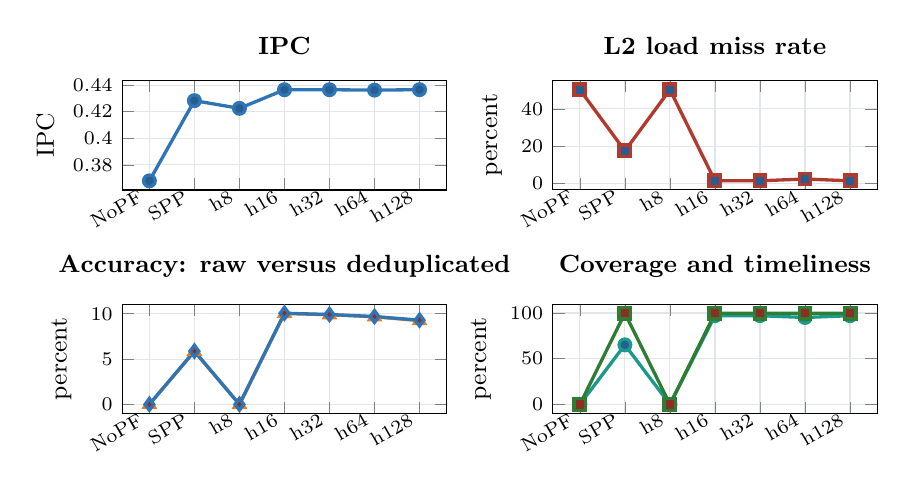
\begin{tikzpicture}
\begin{groupplot}[
  group style={group size=2 by 2,horizontal sep=1.35cm,vertical sep=1.45cm},
  width=0.47\textwidth,height=0.245\textwidth,
  grid=major,grid style={rulegray!70},
  tick label style={font=\scriptsize},label style={font=\small},title style={font=\small\bfseries},
  xtick={0,1,2,3,4,5,6},xticklabels={{NoPF},{SPP},{h8},{h16},{h32},{h64},{h128}},
  x tick label style={rotate=30,anchor=east},
  every axis plot/.append style={very thick,mark size=2.1pt}
]
\nextgroupplot[title={IPC},ylabel={IPC},scaled y ticks=false,
  yticklabel style={/pgf/number format/fixed,/pgf/number format/precision=5}]
\addplot+[color=blue,mark=*] coordinates {(0,0.36800000) (1,0.42834000) (2,0.42255000) (3,0.43654000) (4,0.43656000) (5,0.43626000) (6,0.43660000)};
\nextgroupplot[title={L2 load miss rate},ylabel={percent},scaled y ticks=false]
\addplot+[color=red,mark=square*] coordinates {(0,50.25270955) (1,17.53356473) (2,50.25073042) (3,1.50190862) (4,1.50091906) (5,2.48058602) (6,1.50116645)};
\nextgroupplot[title={Accuracy: raw versus deduplicated},ylabel={percent},scaled y ticks=false]
\addplot+[color=orange,mark=triangle*] coordinates {(0,0) (1,5.86734717) (2,0) (3,10.03375867) (4,9.89178623) (5,9.66944768) (6,9.24046353)};
\addplot+[color=blue,mark=diamond*] coordinates {(0,0) (1,5.87104060) (2,0) (3,10.05752054) (4,9.91539802) (5,9.69233179) (6,9.29338051)};
\nextgroupplot[title={Coverage and timeliness},ylabel={percent},scaled y ticks=false]
\addplot+[color=teal,mark=*] coordinates {(0,0) (1,65.10675377) (2,0) (3,97.00981140) (4,97.01178058) (5,95.06082282) (6,97.01128828)};
\addplot+[color=green,mark=square*] coordinates {(0,0) (1,99.71048584) (2,0) (3,99.63141982) (4,99.63344221) (5,99.63417214) (6,99.63293661)};
\end{groupplot}
\end{tikzpicture}

\vspace{1mm}
{\footnotesize
\textcolor{orange}{Orange triangles}: raw accuracy $A=U/I$;\quad
\textcolor{blue}{blue diamonds}: selected accuracy $A_{\rm sel}=U/(I-Q)$;\quad
\textcolor{teal}{teal circles}: coverage $C$;\quad
\textcolor{green}{green squares}: timeliness $T$.\\
The h8 no-useful point is drawn at zero for visibility; its zero-denominator
timeliness remains \NA\ in the table.}
\end{center}

\section*{3. Quality and traffic---kept separate}
\begin{center}\scriptsize
\resizebox{\textwidth}{!}{%
\begin{tabular}{@{}lrrrrr@{}}
\toprule
Method & raw accuracy $U/I$ & selected accuracy $U/(I-Q)$ & coverage $U/M_0$ & useful/self-miss $U/M$ & timeliness $U/(U+L_t)$ \\
\midrule
Offline SPP & 5.87\% & 5.87\% & 65.11\% & 1.866 & 99.71\% \\
LSTM h8 & 0.00\% & 0.00\% & 0.00\% & 0.000 & \NA \\
LSTM h16 & 10.03\% & 10.06\% & 97.01\% & 32.459 & 99.63\% \\
LSTM h32 & 9.89\% & 9.92\% & 97.01\% & 32.481 & 99.63\% \\
LSTM h64 & 9.67\% & 9.69\% & 95.06\% & 19.258 & 99.63\% \\
LSTM h128 & 9.24\% & 9.29\% & 97.01\% & 32.475 & 99.63\% \\
\bottomrule
\end{tabular}}
\end{center}

\begin{center}\scriptsize
\resizebox{\textwidth}{!}{%
\begin{tabular}{@{}lrrrrrrr@{}}
\toprule
Method & request/L2 load $P/N_L$ & merge/issued $Q/I$ & drop/request $D/P$ & fill/non-merged $F/(I-Q)$ & late/issued $L_t/I$ & useless/issued $W/I$ & resolved-fill utility $U/(U+W)$ \\
\midrule
Offline SPP & 5.576 & 0.06\% & 0.00\% & 5.89\% & 0.02\% & 0.02\% & 99.61\% \\
LSTM h8 & 4.694 & 0.21\% & 0.00\% & 0.00\% & 0.00\% & 0.00\% & \NA \\
LSTM h16 & 4.859 & 0.24\% & 0.00\% & 10.27\% & 0.04\% & 0.20\% & 98.00\% \\
LSTM h32 & 4.928 & 0.24\% & 0.00\% & 10.12\% & 0.04\% & 0.20\% & 98.00\% \\
LSTM h64 & 4.940 & 0.24\% & 0.00\% & 9.89\% & 0.04\% & 0.19\% & 98.04\% \\
LSTM h128 & 5.276 & 0.57\% & 0.00\% & 9.49\% & 0.03\% & 0.19\% & 98.00\% \\
\bottomrule
\end{tabular}}
\end{center}

\begin{center}\scriptsize
\resizebox{\textwidth}{!}{%
\begin{tabular}{@{}lrrrrrrrrr@{}}
\toprule
Method & requested $P$ & dropped $D$ & issued $I$ & PQ merged $Q$ & $I-Q$ & filled $F$ & useful $U$ & useless $W$ & late $L_t$ \\
\midrule
Offline SPP & 2,254,034 & 0 & 2,254,034 & 1,418 & 2,252,616 & 132,785 & 132,252 & 524 & 384 \\
LSTM h8 & 1,897,395 & 0 & 1,897,395 & 3,962 & 1,893,433 & 0 & 0 & 0 & 0 \\
LSTM h16 & 1,963,940 & 0 & 1,963,940 & 4,640 & 1,959,300 & 201,126 & 197,057 & 4,017 & 729 \\
LSTM h32 & 1,992,168 & 0 & 1,992,168 & 4,744 & 1,987,424 & 201,130 & 197,061 & 4,017 & 725 \\
LSTM h64 & 1,996,991 & 0 & 1,996,991 & 4,715 & 1,992,276 & 197,001 & 193,098 & 3,860 & 709 \\
LSTM h128 & 2,132,577 & 0 & 2,132,577 & 12,143 & 2,120,434 & 201,129 & 197,060 & 4,016 & 726 \\
\bottomrule
\end{tabular}}
\end{center}

\begin{infobox}[title={\bfseries Why raw and selected accuracy stay together}]
PQ-merged requests remain in $I$ but are removed from $I-Q$. Here the merge
fractions are below 0.6\%, so raw and selected accuracy differ only slightly.
Selected accuracy is nevertheless never interpreted without raw accuracy,
merge count, coverage, miss rate, traffic, and IPC. In particular, the rise
in h16 useless fills (4,017 versus 524 for SPP) is retained even though h16
has higher selected accuracy.
\end{infobox}




\section*{4. Capacity and h8 diagnosis}
\begin{infobox}[fontupper=\small]
\begin{itemize}[itemsep=1pt,topsep=1pt]
\item h16 is the compact high-performing point: IPC 0.43654 versus 0.42834 for offline SPP (+1.91\%), L2 miss rate falls from 17.53\% to 1.50\%, coverage rises from 65.11\% to 97.01\%, and requests fall by 12.87\%. Timeliness is slightly lower (99.63\% versus 99.71\%), while late and useless counts rise; the result is therefore reported as an outcome/pressure tradeoff rather than a single-score win.
\item h128 is the measured IPC maximum at 0.43660, only 0.00006 above h16 while using 23.17$\times$ as many parameters. h32 is also within 0.00002 of h16. Capacity is non-monotonic at h64, so this one-seed sweep supports practical saturation near h16, not a universal optimum.
\item h8 is not an input, gate, count, target, or replay collapse. Like every
tested capacity, it acts on 100\% of callbacks versus the teacher's 97.24\%;
it has 100\% teacher-trigger recall, 74.86\% target F1, and emits 1.897M
accepted actions. Its distinctive failure is fill selection: every emitted
action is \texttt{FILL\_LLC}, leaving zero \texttt{FILL\_L2}, zero L2
prefetch fills, and zero L2 useful hits.
\item The training action labels are 10.49\% \texttt{FILL\_L2} and 89.51\% \texttt{FILL\_LLC}; evaluation is 10.40\%/89.60\%. The h8 signature is therefore consistent with minority-fill information being lost in the smallest shared representation under the unweighted two-class fill loss. h16 and larger models recover roughly 380k--393k L2 actions, which rules out a global encoder, label, or replayer defect.
\end{itemize}
\end{infobox}

\begin{center}\scriptsize
\resizebox{\textwidth}{!}{%
\begin{tabular}{@{}lrrrrrrrr@{}}
\toprule
Model & predicted trigger & trigger precision & trigger recall & target F1 & matched-fill accuracy & action/teacher & action L2 & action LLC \\
\midrule
LSTM h8 & 100.00\% & 97.24\% & 100.00\% & 74.86\% & 85.36\% & 0.897 & 0 & 1,897,395 \\
LSTM h16 & 100.00\% & 97.24\% & 100.00\% & 74.86\% & 93.49\% & 0.897 & 392,788 & 1,571,152 \\
LSTM h32 & 100.00\% & 97.24\% & 100.00\% & 75.24\% & 93.57\% & 0.909 & 392,788 & 1,599,380 \\
LSTM h64 & 100.00\% & 97.24\% & 100.00\% & 75.32\% & 93.45\% & 0.909 & 379,845 & 1,617,146 \\
LSTM h128 & 100.00\% & 97.24\% & 100.00\% & 77.10\% & 93.94\% & 0.972 & 392,788 & 1,739,789 \\
\bottomrule
\end{tabular}}
\end{center}

\begin{infobox}[title={\bfseries Remaining learned-gate limitation}]
Teacher SPP acts on 97.243\% of evaluation demand callbacks, whereas every
capacity predicts the positive categorical mode on 100\% and is never silent.
Equivalently, 2.757\% of callbacks are silent$\to$act and none are
act$\to$silent. This is a learned argmax operating point, not a probability
threshold or hard-coded degree.
The v2 objective removes the severe v1 under-triggering, but does not make the
gate perfectly calibrated. The report preserves this limitation instead of
equating higher IPC with exact SPP imitation.
\end{infobox}

\section*{5. Provenance and counter cross-check}
Offline SPP reproduces the live reference closely: IPC differs by
$-0.00002$ and measured L2 misses differ by one. The normal and neural lists
are replayed through the same fill-preserving transport. SPP teacher actions
are attached by explicit prior trigger-event identity and are labels only;
they are never neural inference inputs.

\begin{center}\scriptsize
\resizebox{\textwidth}{!}{%
\begin{tabular}{@{}lrrrrrl@{}}
\toprule
Method & $\Delta$L2 loads & $\Delta$L2 misses & $\Delta$PF requests &
$\Delta$useful & $\Delta$late & audit \\
\midrule
Offline SPP & 0 & 0 & 0 & 0 & 0 & exact \\
LSTM h8 & 0 & 0 & 0 & 0 & 0 & exact \\
LSTM h16 & 0 & 0 & 0 & +1 & 0 & recorded $+1$ useful \\
LSTM h32 & 0 & 0 & 0 & +1 & 0 & recorded $+1$ useful \\
LSTM h64 & 0 & 0 & 0 & 0 & 0 & exact \\
LSTM h128 & 0 & 0 & 0 & +1 & 0 & recorded $+1$ useful \\
\bottomrule
\end{tabular}}
\end{center}

Here each delta is \emph{ChampSim final counter minus measurement-event
count}. The primary formulas use the simulator-final counter and never mix
it with the event count; the one-event differences are retained explicitly
rather than assigned an unobserved cause.

\begin{tabularx}{\textwidth}{@{}
  >{\bfseries\raggedright\arraybackslash}p{0.18\textwidth}
  >{\raggedright\arraybackslash}X
  >{\raggedright\arraybackslash}X@{}}
\toprule
Evidence layer & Directly recorded fields & Role in this report \\
\midrule
Chronological source stream &
Demand addresses and raw cache-fill evicted addresses, with content hashes for train, guard, and evaluation. &
Establishes the source-input contract and identical training/inference encoder.\\
Teacher-action audit &
Explicit trigger identity, direct target, fill level, source-call canonicalization, trigger/count/target/fill diagnostics. &
Supervision and behavior diagnosis only; no teacher field is an inference input.\\
Analyzer event stream &
Measurement-window demand loads/hits/misses, PF request events, useful-demand hits, late-demand misses, and requested L2/LLC fill action. &
ROI attribution, h8 fill diagnosis, and independent counter cross-check.\\
ChampSim final statistics &
\texttt{requested}, \texttt{dropped}, \texttt{issued},
\texttt{pq\_merged}, \texttt{filled}, \texttt{useful},
\texttt{useless}, \texttt{late}, L2 loads/misses, cycles, and IPC. &
Source of the primary cache-effect and lifecycle formulas.\\
Live SPP reference &
Measured IPC and demand outcomes. Its final lifecycle counters have a different scope from the offline measurement list. &
Transport-fidelity context only; excluded from primary traffic/accuracy tables.\\
Direct harmful pollution &
No victim identity plus later re-reference outcome is recorded. &
Not claimed; neither low accuracy nor useless/issued is relabeled pollution.\\
\bottomrule
\end{tabularx}

\begin{infobox}[title={\bfseries Reporting decision}]
No additional replay is required to report this v2 single-trace result. h8 is
retained as a measured low-capacity fill failure; h16--h128 establish that the
shared input, label, decoder, and replay path can produce useful L2 actions.
A fresh trace/window and additional seeds are still required before claiming
a general SPP replacement or a universal h16 optimum. Direct harmful-eviction
pollution would require new victim/re-reference instrumentation.
\end{infobox}

{\footnotesize The report uses raw dimensions only. It does not select a
model with the analyzer's legacy balanced-parity field and does not infer
definitions from column names.}

\end{document}
